\documentclass[12pt]{article}
\usepackage{graphicx}
\usepackage{amsmath}
\usepackage{mathtools}
\usepackage{gensymb}
\usepackage{amssymb}
\usepackage{tikz}
\usetikzlibrary{arrows,shapes,automata,petri,positioning,calc}
\usepackage{hyperref}
\usepackage{tikz}
\usetikzlibrary{matrix,calc}
\usepackage[margin=0.5in]{geometry}

\providecommand{\norm}[1]{\left\lVert#1\right\rVert}
\newcommand{\myvec}[1]{\ensuremath{\begin{pmatrix}#1\end{pmatrix}}}
\let\vec\mathbf
%\providecommand $${\norm}[1]{\left\lVert#1\right\rVert}$$
\providecommand{\abs}[1]{\left\vert#1\right\vert}
\let\vec\mathbf

\newcommand{\mydet}[1]{\ensuremath{\begin{vmatrix}#1\end{vmatrix}}}
\providecommand{\brak}[1]{\ensuremath{\left(#1\right)}}
\providecommand{\lbrak}[1]{\ensuremath{\left(#1\right.}}
\providecommand{\rbrak}[1]{\ensuremath{\left.#1\right)}}
\providecommand{\sbrak}[1]{\ensuremath{{}\left[#1\right]}}

\providecommand{\brak}[1]{\ensuremath{\left(#1\right)}}
\providecommand{\norm}[1]{\left\lVert#1\right\rVert}
\newcommand{\solution}{\noindent \textbf{Solution: }}

\let\vec\mathbf
\def\inputGnumericTable{}
\usepackage{color}                                            %%
    \usepackage{array}                                            %%
    \usepackage{longtable}                                        %%
    \usepackage{calc}                                             %%
    \usepackage{multirow}                                         %%
    \usepackage{hhline}                                           %%
    \usepackage{ifthen}
\usepackage{array}
\usepackage{amsmath}   % for having text in math mode
\usepackage{listings}
\lstset{
language=tex,
frame=single, 
breaklines=true
}
\newenvironment{Figure}
  {\par\medskip\noindent\minipage{\linewidth}}
  {\endminipage\par\medskip}
\begin{document}
\begin{center}
\textbf\large{CLASS-9\\CHAPTER-10 \\ CIRCLES}

\end{center}
\section*{Excercise 10.6}

Q1. Prove that the line of centres of two intersecting circles subtends equal angles at the two points of intersection.
\section*{\large Solution}:
\begin{figure}[h!]
\centering
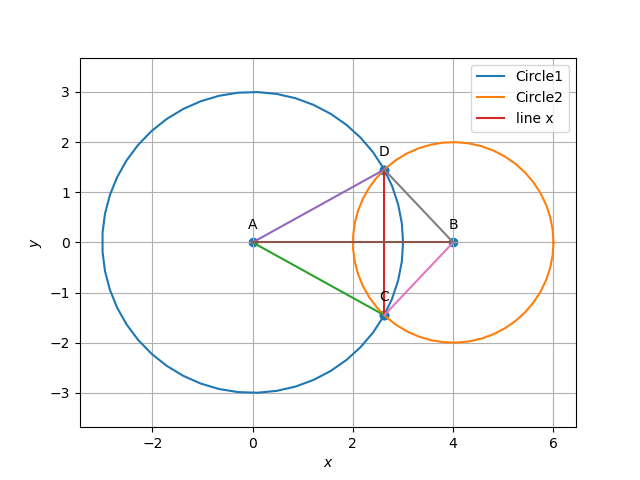
\includegraphics[width=\columnwidth]{figs/circle3.png}
\caption{}
\label{fig:Fig1}
\end{figure}


\section*{\large Construction}:

\begin{table}[h!]
	\small
	\centering
	%\subimport{../tables/}{table1.tex}
     \begin{tabular}{|p{3cm}|p{3cm}|p{3cm}|}
\hline                                        
\textbf{Symbol} & \textbf{Values} & \textbf{Description}\\                                          
\hline                                 
$\theta$ & 30$\degree{}$   & $\angle{BAD} = \angle{BAC}$ \\           
\hline                                    
a &  9 & $AB$ \\     
\hline                      
c & 5 & $AC$ \\
\hline                                     
		$\vec{e}_1$ & $\myvec{
			1\\
			0\\
			}$ & basis vector\\ 
\hline
\end{tabular}

%	\caption{}
	\label{table:table1}
\end{table}


\section*{\large Verification:}

 The two circle equations are given by:
\begin{align}
\label{eq:1}
	\norm{x}^2-9=0\\
	\norm{x}^2-8\vec{e}_1+12=0
\end{align}
Equation of two conics is given by:
 \begin{align}
 \vec{x}^\top\vec{V}_i\vec{x}+2\vec{u}_i^\top\vec{x}+f_i=0, \quad i=1,2
 \label{eq:3}
 \end{align}
 Represent the two circles in conic form:
 \begin{align}
	\vec{x}^\top\vec{x}-9=0\\
	\vec{x}^\top\vec{x}+2\myvec{-4&0}+12=0
\end{align}
On comparing above two equations with \eqref{eq:3}, we get:
 \begin{align}
	  \vec{V}_1&=\vec{I},\vec{u}_1=\myvec{0\\0},f_1=-9\\
	  \vec{V}_2&=\vec{I},\vec{u}_2=\myvec{-4\\0},f_2=12
\end{align}
The intersection of the given conics is obtained
as
\begin{align}
	\label{eq:8}
\vec{V}_1+\mu\vec{V}_2&= \myvec{
\mu+1 & 0\\
0 & \mu+1
}
\\ \label{eq:9}
\vec{u}_1+\mu\vec{u}_2&= \myvec{
4\\
0
}
\\ \label{eq:10}
f_1+\mu f_2&= -21
\end{align}
This conic is a single straight line if and only if, 
\begin{align}
\mydet{\vec{V}_1 + \mu\vec{V}_2 & \vec{u}_1+\mu \vec{u}_2\\ (\vec{u}_1+\mu \vec{u}_2)^{\top} & f_1 + \mu f_2} &= 0
\label{eq:11}
\end{align}
Substituting equation \eqref{eq:8},\eqref{eq:9} and \eqref{eq:10} in equation \eqref{eq:11}:
\begin{align}
\implies \mydet{1+\mu& 0 & -4\mu\\ 
0 & 1+\mu & 0 \\
-4\mu & 0 & -9+12\mu
} &= 0
\end{align}
Solving the above equation we get,
\begin{align}
    \mu = -1
\end{align}
Thus, the parameters for a straight line can be expressed as
 \begin{align}
 \label{eq:14}
	\vec{V} &= 
\vec{V}_1 + \mu\vec{V}_2
=\myvec{ 0 & 0 \\ 0 & 0},
\\ \label{eq:15}
	\vec{u} &=
\vec{u}_1+\mu \vec{u}_2
	= \myvec{
4\\
0
},
\\ \label{eq:16}
f&=f_1 + \mu f_2=-21
\end{align}
The conic equation is given by:
 \begin{align}
 \vec{x}^\top\vec{V}\vec{x}+2\vec{u}^\top\vec{x}+f=0, 
  \label{eq:17}
 \end{align}
By substituting \eqref{eq:14},\eqref{eq:15} and \eqref{eq:16} in conic equation \eqref{eq:17}, we get staright line between the intersection of two circles:
\begin{align}
\myvec{1&0}\vec{x}&=\frac{21}{8}\\
\vec{x}&=\myvec{\frac{21}{8}\\\lambda}\\
\vec{x}&=\myvec{\frac{21}{8}\\0}+\lambda\myvec{0\\1}\label{eq:20}
\end{align}
		Equation \eqref{eq:20} can be expressed in the form of parametric equation
\begin{align}
	\vec{x}=\vec{q}+\lambda\vec{m}\label{eq:21}
\end{align}
The distance form origin to point $\vec{x}$ is given by
\begin{align}
	\norm{\vec{x}}^2&=d^2\label{eq:22}
\end{align}
		Then substituting \eqref{eq:21} in \eqref{eq:22} yeilds,
\begin{align}
	&\implies\brak{\vec{q}+\lambda\vec{m}}^{\top}\brak{\vec{q}+\lambda\vec{m}}=d^2\\
	&\implies \vec{q}^{\top}\vec{q}+\brak{\lambda\vec{m}}^{\top}\lambda\vec{m}+\vec{q}^{\top}\lambda\vec{m}+\brak{\lambda\vec{m}}^{\top}\vec{q}=d^2\\
	&\implies \norm{\vec{q}}^2+\lambda^2\norm{\vec{m}}^2+2\lambda\vec{q}^{\top}\vec{m}=d^2\\
	&\implies \lambda^2\norm{\vec{m}}^2+2\lambda\vec{q}^{\top}\vec{m}+\norm{\vec{q}}^2=d^2\label{eq:26}
\end{align}
where
\begin{align}
	\vec{q}=\myvec{\frac{21}{8}\\0},\vec{m}=\myvec{0\\1} \text{ and } d=r_1=3
	\label{eq:27}
\end{align}
		substituting the values of \eqref{eq:27} in \eqref{eq:26} gives
\begin{align}
	&\implies\lambda^2(1)+2\lambda\myvec{\frac{21}{8}&0}\myvec{0\\1}+\frac{441}{64}=9\\
	&\implies\lambda^2=\frac{135}{64}\\
	&\implies\lambda_i=\pm\frac{3\sqrt{5}}{8}
\end{align}
The intersecting points $\vec{C}$ and $\vec{D}$ are given by:
\begin{align}
    \vec{C}&=\vec{q}+\lambda_1\vec{m}=\myvec{\frac{21}{8}\\[2pt]-\frac{3\sqrt{5}}{8}}\\
    \vec{D}&=\vec{q}+\lambda_2\vec{m}=\myvec{\frac{21}{8}\\[2pt]\frac{3\sqrt{5}}{8}}
\end{align}
		Check whether the intersection angles $\angle$ADB and $\angle$ACB are equal or not:
\begin{enumerate}
\item Finding $\angle$ADB:
	\begin{align}
		 \vec{A-D} = \myvec{-\frac{21}{8}\\[2pt]-\frac{3\sqrt{5}}{8}},
		\vec{B-D}& = \myvec{\frac{11}{8}\\[2pt]-\frac{3\sqrt{5}}{8}}\\
	 \vec{(A-D)^\top(B-D)}&= -\frac{3}{2}\\
	 \norm{\vec{A-D}}\norm{\vec{C-D}}& = 6\\
		\cos(\angle ADB)& = \frac{\vec{(A-D)^\top(B-D)}}{\norm{\vec{A-D}}\norm{\vec{B-D}}}\\
		\angle ADB&=104\degree
\end{align}
\item Finding $\angle$ACB:
\begin{align}
	\vec{A-C} = \myvec{-\frac{21}{8}\\[2pt]\frac{3\sqrt{5}}{8}},
	 \vec{B-C}& = \myvec{\frac{11}{8}\\[2pt]\frac{3\sqrt{5}}{8}}\\
	 \vec{(A-C)^\top(B-C)}&= -\frac{3}{2}\\
	 \norm{\vec{A-C}}\norm{\vec{B-C}}& = 6\\
	 \cos(\angle ACB) &= \frac{\vec{(A-C)^\top(B-C)}}{\norm{\vec{A-C}}\norm{\vec{B-C}}}\\
	 \angle ACB&=104\degree
\end{align}
\end{enumerate}
Hence, both the intersecting angles are equal to each other, which satisfies the above condition.


\end{document}
